\chapter{Limites et Continuité des fonctions}

Ce chapitre aborde l'étude des limites de fonctions aux bornes de leur ensemble de définition, l'étude de la continuité sur un intervalle, et l'application majeure qu'est le Théorème des Valeurs Intermédiaires (TVI).

\section{Limites de Fonctions}

L'étude des limites permet de comprendre le comportement d'une fonction $f$ lorsque sa variable $x$ devient très grande (positivement ou négativement) ou s'approche d'une valeur interdite.

\subsection{Limites à l'infini et asymptotes horizontales}

\begin{definition}[Limite finie à l'infini]
Soit $L \in \R$ et $f$ une fonction définie sur un intervalle $]a, +\infty[$.
On dit que la limite de $f(x)$ lorsque $x$ tend vers $+\infty$ est égale à $L$ si tout intervalle ouvert contenant $L$ contient toutes les valeurs $f(x)$ pour $x$ assez grand. On note alors :
\[
\lim_{x \to +\infty} f(x) = L
\]
Géométriquement, la droite d'équation $y = L$ est appelée \textbf{asymptote horizontale} à la courbe $\mathcal{C}_f$ en $+\infty$.
Une définition analogue s'applique en $-\infty$.
\end{definition}

\begin{definition}[Limite infinie à l'infini]
On dit que la limite de $f(x)$ lorsque $x$ tend vers $+\infty$ est égale à $+\infty$ si, pour tout réel $M > 0$, on a $f(x) > M$ pour $x$ assez grand. On note alors :
\[
\lim_{x \to +\infty} f(x) = +\infty
\]
\end{definition}

\subsection{Limites en un réel $a$ et asymptotes verticales}

\begin{definition}[Limite infinie en un point]
Soit $f$ une fonction définie sur un intervalle $I$ dont $a$ est une borne.
On dit que la limite de $f(x)$ lorsque $x$ tend vers $a$ est égale à $+\infty$ si $f(x)$ devient aussi grand que l'on veut lorsque $x$ est suffisamment proche de $a$. On note :
\[
\lim_{x \to a} f(x) = +\infty
\]
Géométriquement, la droite d'équation $x = a$ est une \textbf{asymptote verticale} à la courbe $\mathcal{C}_f$.
\end{definition}

\subsection{Opérations sur les limites}

Les règles opératoires pour les limites de sommes, produits et quotients de fonctions sont similaires à celles des suites. Cependant, certaines situations conduisent à des \textbf{Formes Indéterminées (F.I.)} où l'on ne peut pas conclure directement :
\[
\text{« } \infty - \infty \text{ », « } 0 \times \infty \text{ », « } \frac{0}{0} \text{ » \ et \ « } \frac{\infty}{\infty} \text{ »}
\]

\subsection{Composition et comparaison de limites}

\begin{theoreme}[Limite d'une fonction composée]
Soient deux fonctions $u$ et $v$. Si :
\[
\lim_{x \to a} u(x) = b \quad \text{et} \quad \lim_{y \to b} v(y) = c
\]
(où $a$, $b$ et $c$ peuvent être des réels ou $\pm\infty$), alors :
\[
\lim_{x \to a} v(u(x)) = c
\]
\end{theoreme}

\begin{theoreme}[Théorème des Gendarmes]
Soient $f$, $g$ et $h$ trois fonctions définies sur un intervalle contenant $a$ (sauf éventuellement en $a$). Supposons que pour tout $x \ne a$ dans cet intervalle :
\[
g(x) \le f(x) \le h(x)
\]
Si $\lim_{x \to a} g(x) = \lim_{x \to a} h(x) = L$ (où $L \in \R$), alors $\lim_{x \to a} f(x) = L$.
\end{theoreme}

\section{Continuité}

\subsection{Définition et propriétés}

La continuité traduit mathématiquement l'idée qu'on peut tracer la courbe représentative d'une fonction « sans lever le crayon ».

\begin{definition}[Continuité en un point]
Soit $f$ une fonction définie sur un intervalle $I$ et $a \in I$.
On dit que $f$ est \textbf{continue en $a$} si :
\[
\lim_{x \to a} f(x) = f(a)
\]
On dit que $f$ est \textbf{continue sur l'intervalle $I$} si $f$ est continue en tout réel de $I$.
\end{definition}

\begin{propriete}[Continuité des fonctions de référence]
Les fonctions affines, puissances, polynômes, rationnelles, trigonométriques ($\sin$, $\cos$), la fonction exponentielle et la fonction racine carrée sont continues sur tout intervalle inclus dans leur ensemble de définition.
\end{propriete}

\subsection{Théorème des valeurs intermédiaires (TVI)}

Le TVI est l'un des théorèmes fondamentaux de l'analyse réelle. Il affirme qu'une fonction continue ne peut pas passer d'une valeur à une autre sans passer par toutes les valeurs intermédiaires.

\begin{theoreme}[Théorème des Valeurs Intermédiaires]
Soit $f$ une fonction continue sur un intervalle $[a, b]$.
Pour tout réel $k$ compris entre $f(a)$ et $f(b)$, il existe au moins un réel $c \in [a, b]$ tel que :
\[
f(c) = k
\]
\end{theoreme}

Dans la pratique, on utilise très souvent son corollaire qui assure l'unicité de la solution.

\begin{theoreme}[Corollaire du TVI (Théorème de la bijection)]
Soit $f$ une fonction continue et \textbf{strictement monotone} sur un intervalle $[a, b]$.
Pour tout réel $k$ compris entre $f(a)$ et $f(b)$, l'équation $f(x) = k$ admet une \textbf{unique} solution $\alpha$ dans l'intervalle $[a, b]$.
\end{theoreme}

Voici une illustration graphique du corollaire du TVI sur un intervalle $[a,b]$ pour une fonction strictement croissante :

\begin{center}
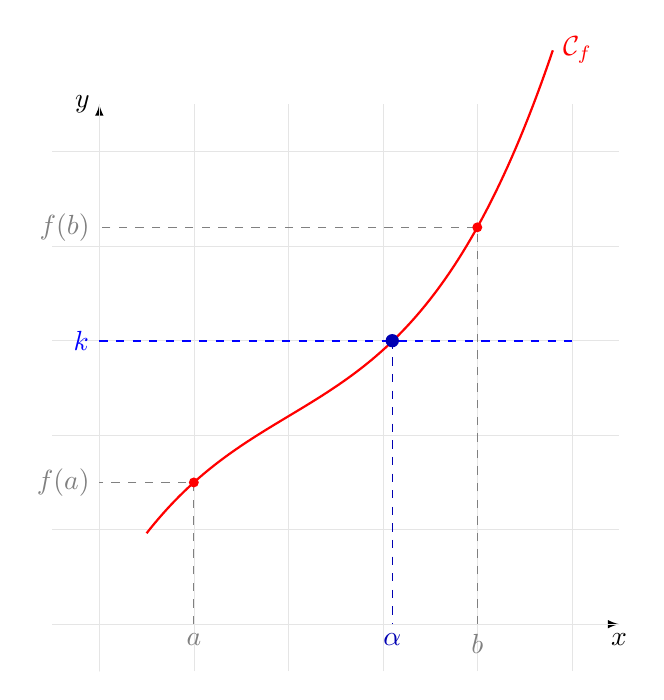
\begin{tikzpicture}[scale=1.2]
  % Axes
  \draw[->,>=latex] (-0.5,0) -- (5.5,0) node[below] {$x$};
  \draw[->,>=latex] (0,-0.5) -- (0,5.5) node[left] {$y$};
  \draw[gray!20,very thin] (-0.5,-0.5) grid (5.5,5.5);
  
  % Courbe strictement croissante
  \draw[domain=0.5:4.8, samples=100, color=red, thick] plot (\x, {0.1*\x^3 - 0.6*\x^2 + 1.8*\x + 0.2}) node[right] {$\mathcal{C}_f$};
  
  % Bornes de l'intervalle
  \coordinate (A) at (1, 1.5);
  \coordinate (B) at (4, 4.2);
  
  \draw[dashed, gray] (1,0) node[below] {$a$} -- (1,1.5) -- (0,1.5) node[left] {$f(a)$};
  \draw[dashed, gray] (4,0) node[below] {$b$} -- (4,4.2) -- (0,4.2) node[left] {$f(b)$};
  
  % Ligne de niveau k et solution unique alpha
  \draw[dashed, blue, thick] (0,3) node[left, color=blue] {$k$} -- (5,3);
  \draw[dashed, blue!70!black] (3.1,3) -- (3.1,0) node[below, color=blue!70!black] {$\alpha$};
  \fill[blue!70!black] (3.1,3) circle (2pt);
  
  % Points remarquables sur la courbe
  \fill[red] (1,1.5) circle (1.5pt);
  \fill[red] (4,4.2) circle (1.5pt);
\end{tikzpicture}
\end{center}

\section{Fonctions Réciproques et Applications}

Le corollaire du TVI (ou théorème de la bijection) montre qu'une fonction continue et strictement monotone réalise une correspondance univoque. Cela permet de définir sa fonction réciproque.

\subsection{Théorème de la bijection et fonction réciproque}

\begin{theoreme}[Théorème de la bijection]
Soit $f$ une fonction continue et strictement monotone sur un intervalle $I$.
Alors, $f$ réalise une bijection de l'intervalle $I$ sur l'intervalle image $J = f(I)$.
Cela signifie que pour tout $y \in J$, l'équation $f(x) = y$ admet une unique solution $x \in I$.
On peut alors définir la \textbf{fonction réciproque} de $f$, notée $f^{-1}$, qui à tout $y \in J$ associe ce réel unique $x \in I$ :
\[
x = f^{-1}(y) \iff y = f(x)
\]
\end{theoreme}

\begin{propriete}[Propriétés de la fonction réciproque]
Soit $f$ une bijection continue d'un intervalle $I$ sur $J = f(I)$.
\begin{itemize}
    \item La fonction $f^{-1}$ est continue sur $J$.
    \item La fonction $f^{-1}$ a le même sens de variation que $f$ sur $J$.
    \item Pour tout $x \in I$, $(f^{-1} \circ f)(x) = x$, et pour tout $y \in J$, $(f \circ f^{-1})(y) = y$.
    \item Les courbes représentatives $\mathcal{C}_f$ et $\mathcal{C}_{f^{-1}}$ dans un repère orthonormé sont symétriques par rapport à la première bissectrice, c'est-à-dire la droite d'équation $y = x$.
\end{itemize}
\end{propriete}

\subsection{La fonction racine $n$-ième}

\begin{definition}[Racine $n$-ième]
Soit $n \in \N^* \setminus \{1\}$.
La fonction $f: x \mapsto x^n$ est continue et strictement croissante sur $[0, +\infty[$. Elle réalise donc une bijection de $[0, +\infty[$ sur $[0, +\infty[$.
Sa fonction réciproque est appelée la \textbf{fonction racine $n$-ième}, notée $x \mapsto \sqrt[n]{x}$ ou $x \mapsto x^{1/n}$ :
\[
y = \sqrt[n]{x} \iff y^n = x \quad (\text{avec } x \ge 0 \text{ et } y \ge 0)
\]
\end{definition}

\begin{propriete}[Propriétés de calcul]
Pour tous réels positifs $x$ et $y$, et tous entiers naturels non nuls $p$ et $q$ (supérieurs ou égaux à 2) :
\begin{itemize}
    \item $\sqrt[n]{x^n} = x$ \quad et \quad $(\sqrt[n]{x})^n = x$.
    \item $\sqrt[n]{xy} = \sqrt[n]{x} \times \sqrt[n]{y}$.
    \item $\sqrt[n]{\frac{x}{y}} = \frac{\sqrt[n]{x}}{\sqrt[n]{y}}$ \quad (pour $y > 0$).
    \item $\sqrt[n]{x^m} = (\sqrt[n]{x})^m$.
    \item $\sqrt[n]{\sqrt[m]{x}} = \sqrt[nm]{x}$.
\end{itemize}
\end{propriete}

\begin{propriete}[Limites]
La fonction racine $n$-ième est strictement croissante et continue sur $[0, +\infty[$. De plus :
\[
\lim_{x \to +\infty} \sqrt[n]{x} = +\infty
\]
\end{propriete}

\subsection{La fonction Arctangente}

\begin{definition}[Fonction Arctangente]
La fonction tangente $x \mapsto \tan(x) = \frac{\sin(x)}{\cos(x)}$ est continue et strictement croissante sur l'intervalle ouvert $I = \left]-\frac{\pi}{2}, \frac{\pi}{2}\right[$.
Elle réalise une bijection de $\left]-\frac{\pi}{2}, \frac{\pi}{2}\right[$ sur $J = \R$.
Sa fonction réciproque est appelée la \textbf{fonction Arctangente}, notée $\arctan$ :
\[
y = \arctan(x) \iff x = \tan(y) \quad \left(\text{avec } x \in \R \text{ et } y \in \left]-\frac{\pi}{2}, \frac{\pi}{2}\right[\right)
\]
\end{definition}

\begin{propriete}[Propriétés de la fonction Arctangente]
\begin{itemize}
    \item La fonction $\arctan$ est continue et strictement croissante sur $\R$.
    \item Elle est impaire : pour tout $x \in \R$, $\arctan(-x) = -\arctan(x)$.
    \item Limites aux bornes :
    \[
    \lim_{x \to +\infty} \arctan(x) = \frac{\pi}{2} \quad \text{et} \quad \lim_{x \to -\infty} \arctan(x) = -\frac{\pi}{2}
    \]
    Les droites d'équation $y = \frac{\pi}{2}$ et $y = -\frac{\pi}{2}$ sont des asymptotes horizontales à la courbe de $\arctan$ en $+\infty$ et $-\infty$.
    \item Relations fondamentales :
    \[
    \text{Pour tout } x \in \R, \ \tan(\arctan(x)) = x
    \]
    \[
    \text{Pour tout } x \in \left]-\frac{\pi}{2}, \frac{\pi}{2}\right[, \ \arctan(\tan(x)) = x
    \]
    \item Valeurs remarquables à connaître :
    \begin{center}
    \renewcommand{\arraystretch}{1.5}
    \begin{tabular}{|c|c|c|c|c|c|}
    \hline
    $x$ & $0$ & $\frac{\sqrt{3}}{3}$ & $1$ & $\sqrt{3}$ \\
    \hline
    $\arctan(x)$ & $0$ & $\frac{\pi}{6}$ & $\frac{\pi}{4}$ & $\frac{\pi}{3}$ \\
    \hline
    \end{tabular}
    \end{center}
    \item Pour tout $x > 0$, $\arctan(x) + \arctan\left(\frac{1}{x}\right) = \frac{\pi}{2}$.
\end{itemize}
\end{propriete}

\section{Méthodes Clés}

\begin{methode}[Lever une indétermination en $+\infty$]
Pour lever une indétermination sur une fonction rationnelle ou polynomiale en $+\infty$ ou $-\infty$, la méthode standard consiste à **mettre en facteur le terme de plus haut degré** au numérateur et au dénominateur.
\end{methode}

\begin{exemple}[Calcul de limite]
Calculons la limite suivante :
\[
\lim_{x \to +\infty} \frac{2x^2 - x + 1}{x^2 + 3}
\]
C'est une forme indéterminée du type « $\frac{\infty}{\infty}$ ». Déterminons sa limite en factorisant :
\[
\frac{2x^2 - x + 1}{x^2 + 3} = \frac{x^2 \left(2 - \frac{1}{x} + \frac{1}{x^2}\right)}{x^2 \left(1 + \frac{3}{x^2}\right)} = \frac{2 - \frac{1}{x} + \frac{1}{x^2}}{1 + \frac{3}{x^2}}
\]
Comme $\lim_{x \to +\infty} \frac{1}{x} = 0$ et $\lim_{x \to +\infty} \frac{1}{x^2} = 0$, on obtient par quotient :
\[
\lim_{x \to +\infty} \frac{2x^2 - x + 1}{x^2 + 3} = \frac{2}{1} = 2
\]
\end{exemple}

\section{Approximation par Dichotomie}

La méthode de **dichotomie** (ou de bissection) est une méthode d'analyse numérique permettant de déterminer des valeurs approchées de l'unique solution $\alpha$ d'une équation du type $f(x) = k$ sur un intervalle $[a, b]$, où $f$ est une fonction continue et strictement monotone.

Elle repose directement sur le théorème des valeurs intermédiaires (TVI).

\begin{definition}[Principe de la dichotomie]
Soit $f$ une fonction continue et strictement croissante sur $[a, b]$ telle que $f(a) < k < f(b)$. L'équation $f(x) = k$ admet une unique solution $\alpha \in ]a, b[$.
Pour approcher $\alpha$ avec une précision $\epsilon > 0$ donnée :
\begin{enumerate}
    \item On calcule le milieu de l'intervalle $m = \frac{a+b}{2}$.
    \item On évalue $f(m)$ :
    \begin{itemize}
        \item Si $f(m) < k$, alors $\alpha \in ]m, b[$. Le nouvel intervalle d'étude devient $[m, b]$.
        \item Si $f(m) > k$, alors $\alpha \in ]a, m[$. Le nouvel intervalle d'étude devient $[a, m]$.
    \end{itemize}
    \item On répète l'opération sur le nouvel intervalle jusqu'à ce que la largeur de l'intervalle soit inférieure ou égale à $\epsilon$ (soit $b - a \le \epsilon$).
\end{enumerate}
\end{definition}

\begin{exemple}[Calcul manuel par dichotomie]
Soit la fonction $f(x) = x^3 + x - 3$ sur $[1, 2]$. Elle est continue et strictement croissante. On cherche à encadrer la solution $\alpha$ de $f(x) = 0$ à la précision $\epsilon = 0,25$.
\begin{itemize}
    \item **Étape 0** : L'intervalle initial est $[1, 2]$ de longueur $1 > 0,25$. On a $f(1) = -1 < 0$ et $f(2) = 7 > 0$.
    \item **Étape 1** : Le milieu de $[1, 2]$ est $m_1 = 1,5$.
    \[
    f(1,5) = (1,5)^3 + 1,5 - 3 = 3,375 + 1,5 - 3 = 1,875 > 0
    \]
    Puisque $f(1) < 0$ et $f(1,5) > 0$, la solution $\alpha$ appartient à $[1 \,; 1,5]$.
    La longueur du nouvel intervalle est $1,5 - 1 = 0,5 > 0,25$.
    \item **Étape 2** : Le milieu de $[1 \,; 1,5]$ est $m_2 = 1,25$.
    \[
    f(1,25) = (1,25)^3 + 1,25 - 3 = 1,953125 + 1,25 - 3 = 0,203125 > 0
    \]
    Puisque $f(1) < 0$ et $f(1,25) > 0$, la solution $\alpha$ appartient à $[1 \,; 1,25]$.
    La longueur de ce nouvel intervalle est $1,25 - 1 = 0,25 \le \epsilon$.
\end{itemize}
On s'arrête ici. L'encadrement cherché est donc :
\[
1 \le \alpha \le 1,25
\]
\end{exemple}

\section{Exercices d'Entraînement Résolus}

\subsection*{Exercice 1 : Levée d'indétermination par simplification}
Déterminer la limite en 2 de la fonction $f$ définie sur $\R \setminus \{1; 2\}$ par :
\[
f(x) = \frac{x^2 - 4}{x^2 - 3x + 2}
\]

\textbf{Solution :}
En évaluant directement en $x=2$, on obtient une forme indéterminée du type « $\frac{0}{0}$ ».
Factorisons le numérateur et le dénominateur :
- Le numérateur est une différence de carrés : $x^2 - 4 = (x-2)(x+2)$.
- Le dénominateur $x^2 - 3x + 2$ admet pour racine évidente 2 (car $2^2 - 3(2) + 2 = 0$). L'autre racine est 1. On peut donc factoriser par $x^2 - 3x + 2 = (x-2)(x-1)$.
Pour tout $x \in \R \setminus \{1; 2\}$, simplifions l'expression :
\[
f(x) = \frac{(x-2)(x+2)}{(x-2)(x-1)} = \frac{x+2}{x-1}
\]
Ainsi :
\[
\lim_{x \to 2} f(x) = \lim_{x \to 2} \frac{x+2}{x-1} = \frac{2+2}{2-1} = 4
\]

\subsection*{Exercice 2 : Levée d'indétermination par quantité conjuguée}
Déterminer la limite en $+\infty$ de la fonction $f$ définie sur $[0, +\infty[$ par :
\[
f(x) = \sqrt{x^2 + x} - x
\]

\textbf{Solution :}
C'est une forme indéterminée du type « $\infty - \infty$ ». Utilisons l'expression conjuguée :
\[
f(x) = \frac{\left(\sqrt{x^2+x}-x\right)\left(\sqrt{x^2+x}+x\right)}{\sqrt{x^2+x}+x} = \frac{(x^2+x) - x^2}{\sqrt{x^2+x}+x} = \frac{x}{\sqrt{x^2\left(1 + \frac{1}{x}\right)}+x}
\]
Pour $x > 0$, $\sqrt{x^2} = x$, donc :
\[
f(x) = \frac{x}{x\sqrt{1+\frac{1}{x}}+x} = \frac{x}{x\left(\sqrt{1+\frac{1}{x}}+1\right)} = \frac{1}{\sqrt{1+\frac{1}{x}}+1}
\]
Comme $\lim_{x \to +\infty} \frac{1}{x} = 0$, on a par limite de somme et de quotient :
\[
\lim_{x \to +\infty} f(x) = \frac{1}{\sqrt{1+0}+1} = \frac{1}{2}
\]

\subsection*{Exercice 3 : Limite de fonctions trigonométriques par encadrement}
Déterminer la limite en $+\infty$ de la fonction $f$ définie sur $]0, +\infty[$ par :
\[
f(x) = \frac{\cos(x)}{x}
\]

\textbf{Solution :}
Pour tout réel $x > 0$, on sait que $-1 \le \cos(x) \le 1$.
En divisant par $x$ (qui est strictement positif), on obtient :
\[
-\frac{1}{x} \le \frac{\cos(x)}{x} \le \frac{1}{x}
\]
Or, $\lim_{x \to +\infty} -\frac{1}{x} = 0$ et $\lim_{x \to +\infty} \frac{1}{x} = 0$.
D'après le théorème des Gendarmes, on en déduit :
\[
\lim_{x \to +\infty} f(x) = 0
\]

\subsection*{Exercice 4 : Recherche d'asymptotes}
Déterminer les asymptotes à la courbe représentative de la fonction $f$ définie sur $]1, +\infty[$ par :
\[
f(x) = \frac{2x+3}{x-1}
\]

\textbf{Solution :}
\begin{itemize}
    \item \textbf{Limite en $1^+$} : Le numérateur tend vers $2(1)+3 = 5$. Le dénominateur tend vers $0^+$. Par quotient :
    \[
    \lim_{x \to 1^+} f(x) = +\infty
    \]
    La droite d'équation $x = 1$ est donc une **asymptote verticale** à la courbe $\mathcal{C}_f$.
    
    \item \textbf{Limite en $+\infty$} : Factorisons par $x$ au numérateur et au dénominateur :
    \[
    f(x) = \frac{x\left(2 + \frac{3}{x}\right)}{x\left(1 - \frac{1}{x}\right)} = \frac{2 + \frac{3}{x}}{1 - \frac{1}{x}}
    \]
    Puisque $\lim_{x \to +\infty} \frac{1}{x} = 0$, on a par quotient :
    \[
    \lim_{x \to +\infty} f(x) = \frac{2+0}{1-0} = 2
    \]
    La droite d'équation $y = 2$ est donc une **asymptote horizontale** à la courbe $\mathcal{C}_f$ en $+\infty$.
\end{itemize}

\subsection*{Exercice 5 : Étude de la continuité en un point}
Soit la fonction $f$ définie sur $\R$ par :
\[
f(x) = 
\begin{cases} 
2x + 1 & \text{si } x \le 1 \\
x^2 + 2 & \text{si } x > 1
\end{cases}
\]
La fonction $f$ est-elle continue en 1 ?

\textbf{Solution :}
La fonction $f$ est continue en 1 si et seulement si $\lim_{x \to 1^-} f(x) = \lim_{x \to 1^+} f(x) = f(1)$.
- Calculons $f(1)$ : par définition pour $x \le 1$, $f(1) = 2(1) + 1 = 3$.
- Limite à gauche en 1 : $\lim_{x \to 1^-} f(x) = \lim_{x \to 1^-} (2x+1) = 3$.
- Limite à droite en 1 : $\lim_{x \to 1^+} f(x) = \lim_{x \to 1^+} (x^2+2) = 1^2 + 2 = 3$.
Puisque $\lim_{x \to 1^-} f(x) = \lim_{x \to 1^+} f(x) = f(1) = 3$, la fonction $f$ est **continue en 1**.

\subsection*{Exercice 6 : Application du théorème des valeurs intermédiaires}
Démontrer que l'équation $x^3 + 3x - 5 = 0$ admet au moins une solution réelle dans l'intervalle $[1, 2]$.

\textbf{Solution :}
Soit la fonction $f$ définie sur $[1, 2]$ par $f(x) = x^3 + 3x - 5$.
- $f$ est une fonction polynomiale, elle est donc continue sur $[1, 2]$.
- Calculons les valeurs aux bornes :
  - $f(1) = 1^3 + 3(1) - 5 = 1 + 3 - 5 = -1$.
  - $f(2) = 2^3 + 3(2) - 5 = 8 + 6 - 5 = 9$.
- On constate que $f(1) < 0$ et $f(2) > 0$. Le nombre 0 est donc compris entre $f(1)$ et $f(2)$.
D'après le Théorème des Valeurs Intermédiaires (TVI), il existe au moins un réel $c \in [1, 2]$ tel que $f(c) = 0$.
L'équation admet donc au moins une solution sur $[1,2]$.

\subsection*{Exercice 7 : Continuité par définition de limite}
Démontrer que la fonction $f(x) = \frac{1}{x}$ est continue en tout point $a > 0$ en revenant à la définition.

\textbf{Solution :}
Pour tout $a > 0$, calculons la limite de $f(x)$ quand $x$ tend vers $a$ :
\[
\lim_{x \to a} f(x) = \lim_{x \to a} \frac{1}{x} = \frac{1}{a}
\]
Puisque la limite de $f(x)$ quand $x \to a$ existe et vaut précisément $f(a) = \frac{1}{a}$, la fonction $f$ est continue en $a$. Comme cela est vrai pour tout $a > 0$, la fonction $f$ est continue sur l'intervalle $]0, +\infty[$.

\subsection*{Exercice 8 : Limite d'une fonction composée}
Déterminer la limite en $0^+$ de la fonction $h(x) = \cos(\sqrt{x})$.

\textbf{Solution :}
La fonction $h$ est la composée de $u(x) = \sqrt{x}$ et de $v(y) = \cos(y)$.
1. Cherchons la limite de $u(x)$ en $0^+$ :
   \[
   \lim_{x \to 0^+} \sqrt{x} = 0
   \]
2. Cherchons la limite de $v(y)$ en 0 :
   \[
   \lim_{y \to 0} \cos(y) = \cos(0) = 1
   \]
D'après le théorème de la limite d'une fonction composée, on conclut :
\[
\lim_{x \to 0^+} \cos(\sqrt{x}) = 1
\]

\subsection*{Exercice 9 : Limite oscillante amortie}
Déterminer la limite en $0^+$ de la fonction $f$ définie sur $]0, +\infty[$ par :
\[
f(x) = x \sin\left(\frac{1}{x}\right)
\]

\textbf{Solution :}
Pour tout $x > 0$, $-1 \le \sin\left(\frac{1}{x}\right) \le 1$.
En multipliant par $x$ (qui est strictement positif) :
\[
-x \le x \sin\left(\frac{1}{x}\right) \le x
\]
Or, $\lim_{x \to 0^+} -x = 0$ et $\lim_{x \to 0^+} x = 0$.
D'après le théorème des Gendarmes, la limite en $0^+$ de $f(x)$ est :
\[
\lim_{x \to 0^+} x \sin\left(\frac{1}{x}\right) = 0
\]

\subsection*{Exercice 10 : Continuité globale et paramètre}
Déterminer la valeur du réel $a$ pour laquelle la fonction $f$ définie sur $\R$ par :
\[
f(x) = 
\begin{cases} 
3x + a & \text{si } x < 2 \\
x^2 - 1 & \text{si } x \ge 2
\end{cases}
\]
est continue sur $\R$.

\textbf{Solution :}
Les fonctions $x \mapsto 3x+a$ et $x \mapsto x^2-1$ sont des polynômes, donc continues sur $]-\infty, 2[$ et $]2, +\infty[$ respectivement, quelle que soit la valeur de $a$.
La fonction $f$ est continue sur $\R$ si et seulement si elle est continue en 2, soit $\lim_{x \to 2^-} f(x) = f(2)$.
- $f(2) = 2^2 - 1 = 3$.
- $\lim_{x \to 2^+} f(x) = \lim_{x \to 2^+} (x^2-1) = 3$.
- $\lim_{x \to 2^-} f(x) = \lim_{x \to 2^-} (3x+a) = 3(2) + a = 6 + a$.
Pour assurer la continuité, on doit avoir :
\[
6 + a = 3 \iff a = -3
\]

\subsection*{Exercice 11 : Calcul de limite avec racine troisième}
Déterminer la limite en $+\infty$ de la fonction suivante :
\[
f(x) = \sqrt[3]{x^3 + x^2} - x
\]

\textbf{Solution :}
C'est une forme indéterminée de la forme « $\infty - \infty$ ». Utilisons l'identité algébrique $a^3 - b^3 = (a-b)(a^2 + ab + b^2)$, qui donne $a-b = \frac{a^3 - b^3}{a^2 + ab + b^2}$.
Ici, posons $a = \sqrt[3]{x^3+x^2}$ et $b = x$. On a :
\[
f(x) = \frac{(x^3 + x^2) - x^3}{(\sqrt[3]{x^3 + x^2})^2 + x\sqrt[3]{x^3 + x^2} + x^2} = \frac{x^2}{(\sqrt[3]{x^3(1 + 1/x)})^2 + x\sqrt[3]{x^3(1 + 1/x)} + x^2}
\]
Puisque $\sqrt[3]{x^3} = x$ pour $x > 0$, on a :
\[
f(x) = \frac{x^2}{x^2(\sqrt[3]{1 + 1/x})^2 + x^2\sqrt[3]{1 + 1/x} + x^2} = \frac{x^2}{x^2 \left( (\sqrt[3]{1 + 1/x})^2 + \sqrt[3]{1 + 1/x} + 1 \right)}
\]
Pour $x > 0$, on simplifie par $x^2$ :
\[
f(x) = \frac{1}{(\sqrt[3]{1 + 1/x})^2 + \sqrt[3]{1 + 1/x} + 1}
\]
Puisque $\lim_{x\to +\infty} \frac{1}{x} = 0$, on obtient par limite de somme et de quotient :
\[
\lim_{x \to +\infty} f(x) = \frac{1}{1^2 + 1 + 1} = \frac{1}{3}
\]

\subsection*{Exercice 12 : Simplification avec la fonction Arctangente}
Démontrer que pour tout $x > 0$ :
\[
\arctan(x) + \arctan\left(\frac{1}{x}\right) = \frac{\pi}{2}
\]

\textbf{Solution :}
Soit $x > 0$. Posons $\theta = \arctan(x)$.
Puisque $x > 0$, on a $\theta \in \left]0, \frac{\pi}{2}\right[$.
On a $\tan(\theta) = x$.
Étudions le nombre $\frac{\pi}{2} - \theta$. Comme $\theta \in \left]0, \frac{\pi}{2}\right[$, on a également $\frac{\pi}{2} - \theta \in \left]0, \frac{\pi}{2}\right[$.
Calculons la tangente de cet angle en utilisant la formule trigonométrique $\tan\left(\frac{\pi}{2} - \theta\right) = \frac{1}{\tan(\theta)}$ :
\[
\tan\left(\frac{\pi}{2} - \theta\right) = \frac{1}{\tan(\theta)} = \frac{1}{x}
\]
Ainsi, $\frac{\pi}{2} - \theta$ est l'unique angle dans $\left]-\frac{\pi}{2}, \frac{\pi}{2}\right[$ dont la tangente vaut $\frac{1}{x}$.
Par définition de la fonction Arctangente, on a donc :
\[
\arctan\left(\frac{1}{x}\right) = \frac{\pi}{2} - \theta = \frac{\pi}{2} - \arctan(x)
\]
Ce qui donne bien :
\[
\arctan(x) + \arctan\left(\frac{1}{x}\right) = \frac{\pi}{2}
\]

\section{Problèmes Résolus}

\subsection*{Problème 1 : Étude complète et résolution approchée par dichotomie}
Soit la fonction $f$ définie sur $\R$ par :
\[
f(x) = x^3 - 3x - 1
\]
\begin{enumerate}
    \item Dresser le tableau de variations complet de $f$ sur $\R$.
    \item Montrer que l'équation $f(x) = 0$ admet exactement trois solutions réelles $\alpha, \beta, \gamma$ que l'on localisera dans des intervalles de longueur 1.
    \item On s'intéresse à la solution positive $\gamma$. Démontrer que $\gamma \in [1, 2]$.
    \item Simuler les trois premières étapes de l'algorithme de dichotomie sur l'intervalle $[1, 2]$ pour déterminer un encadrement plus précis de $\gamma$.
\end{enumerate}

\textbf{Solution :}
\begin{enumerate}
    \item La fonction $f$ est polynomiale, donc dérivable sur $\R$. Sa dérivée est :
    \[
    f'(x) = 3x^2 - 3 = 3(x^2 - 1) = 3(x-1)(x+1)
    \]
    Le signe de $f'(x)$ est positif à l'extérieur des racines $-1$ et $1$, et négatif entre elles.
    - Limites : $\lim_{x \to -\infty} f(x) = \lim_{x \to -\infty} x^3 = -\infty$ et $\lim_{x \to +\infty} f(x) = +\infty$.
    - Extremums : $f(-1) = (-1)^3 - 3(-1) - 1 = -1 + 3 - 1 = 1$ et $f(1) = 1^3 - 3(1) - 1 = -3$.
    Ainsi, $f$ est strictement croissante sur $]-\infty, -1]$, strictement décroissante sur $[-1, 1]$, et strictement croissante sur $[1, +\infty[$.
    
    \item Appliquons le corollaire du TVI sur trois intervalles :
    - Sur $]-\infty, -1]$ : $f$ est continue et strictement croissante. L'image de cet intervalle est $]-\infty, 1]$. Comme $0 \in ]-\infty, 1]$, il existe une unique solution $\alpha \in ]-\infty, -1]$. Comme $f(-2) = -8+6-1 = -3 < 0$, on a $\alpha \in [-2, -1]$.
    - Sur $[-1, 1]$ : $f$ est continue et strictement décroissante. $f(-1) = 1 > 0$ et $f(1) = -3 < 0$. Comme 0 est compris entre $-3$ et 1, il existe une unique solution $\beta \in [-1, 1]$. Comme $f(0) = -1 < 0$, on a $\beta \in [-1, 0]$.
    - Sur $[1, +\infty[$ : $f$ est continue et strictement croissante. L'image est $[-3, +\infty[$. Comme $0 \in [-3, +\infty[$, il existe une unique solution $\gamma \in [1, +\infty[$. Comme $f(2) = 8-6-1 = 1 > 0$, on a $\gamma \in [1, 2]$.
    L'équation $f(x)=0$ possède donc exactement trois solutions réelles.
    
    \item D'après la question précédente, $f(1) = -3 < 0$ et $f(2) = 1 > 0$. La fonction étant continue et strictement croissante sur $[1, 2]$, la solution unique $\gamma$ appartient bien à $[1, 2]$.
    
    \item Appliquons l'algorithme de dichotomie sur $[a, b] = [1, 2]$ :
    - \textbf{Étape 1} : Le milieu est $m_1 = \frac{1+2}{2} = 1,5$.
      Calculons $f(1,5) = 1,5^3 - 3(1,5) - 1 = 3,375 - 4,5 - 1 = -2,125 < 0$.
      Comme $f(1,5) < 0$ et $f(2) > 0$, la solution $\gamma$ est dans $[1,5; 2]$.
    - \textbf{Étape 2} : Le nouveau milieu est $m_2 = \frac{1,5+2}{2} = 1,75$.
      Calculons $f(1,75) = 1,75^3 - 3(1,75) - 1 = 5,359 - 5,25 - 1 = -0,891 < 0$.
      Comme $f(1,75) < 0$ et $f(2) > 0$, la solution $\gamma$ est dans $[1,75; 2]$.
    - \textbf{Étape 3} : Le nouveau milieu est $m_3 = \frac{1,75+2}{2} = 1,875$.
      Calculons $f(1,875) = 1,875^3 - 3(1,875) - 1 \approx 6,592 - 5,625 - 1 = -0,033 < 0$.
      Comme $f(1,875) < 0$ et $f(2) > 0$, la solution $\gamma$ est dans $[1,875; 2]$.
    Ainsi, à l'issue de ces 3 étapes, on obtient l'encadrement : $1,875 < \gamma < 2$.
\end{enumerate}

\subsection*{Problème 2 : Le théorème du point fixe}
Soit $f$ une fonction continue d'un intervalle $[0, 1]$ dans lui-même (c'est-à-dire que pour tout $x \in [0, 1]$, $f(x) \in [0, 1]$).
\begin{enumerate}
    \item Soit $g$ la fonction définie sur $[0, 1]$ par $g(x) = f(x) - x$.
    Montrer que $g(0) \ge 0$ et $g(1) \le 0$.
    \item En déduire qu'il existe au moins un réel $c \in [0, 1]$ tel que $f(c) = c$. (Un tel point est appelé un \textbf{point fixe} de $f$).
    \item Application : Démontrer que la fonction $f(x) = \cos(x)$ admet au moins un point fixe sur l'intervalle $[0, \pi/2]$.
\end{enumerate}

\textbf{Solution :}
\begin{enumerate}
    \item Par hypothèse, pour tout $x \in [0, 1]$, $f(x) \in [0, 1]$, donc $0 \le f(x) \le 1$.
    - Pour $x = 0$ : $g(0) = f(0) - 0 = f(0)$. Comme $f(0) \ge 0$, on a bien $g(0) \ge 0$.
    - Pour $x = 1$ : $g(1) = f(1) - 1$. Comme $f(1) \le 1$, on a bien $f(1) - 1 \le 0 \implies g(1) \le 0$.
    
    \item La fonction $f$ est continue sur $[0, 1]$, et la fonction $x \mapsto x$ l'est également. Par différence, la fonction $g$ est continue sur $[0, 1]$.
    On a $g(0) \ge 0$ et $g(1) \le 0$. Le nombre 0 est donc compris entre $g(1)$ et $g(0)$.
    D'après le Théorème des Valeurs Intermédiaires (TVI), il existe au moins un réel $c \in [0, 1]$ tel que $g(c) = 0$.
    Or, $g(c) = 0 \iff f(c) - c = 0 \iff f(c) = c$.
    Il existe donc bien un point fixe $c \in [0, 1]$ pour la fonction $f$.
    
    \item Soit la fonction $f(x) = \cos(x)$ sur $[0, \pi/2]$.
    Puisque pour tout $x \in [0, \pi/2]$, $\cos(x) \in [0, 1] \subset [0, \pi/2]$ (car $\pi/2 \approx 1,57 > 1$), $f$ envoie bien $[0, \pi/2]$ dans lui-même.
    La fonction $f$ étant continue sur $[0, \pi/2]$, on peut appliquer le théorème précédent (adapté à l'intervalle $[0, \pi/2]$).
    Il existe donc au moins un réel $c \in [0, \pi/2]$ tel que $\cos(c) = c$.
\end{enumerate}

\subsection*{Problème 3 : Prolongement par continuité}
Soit la fonction $f$ définie sur l'intervalle $]0, +\infty[$ par :
\[
f(x) = \frac{\sqrt{x+1} - 1}{x}
\]
\begin{enumerate}
    \item Montrer que la fonction $f$ n'est pas définie en 0.
    \item Déterminer la limite de $f(x)$ lorsque $x$ tend vers 0 (par valeurs supérieures).
    \item En déduire qu'il est possible de prolonger la fonction $f$ par continuité en 0. Définir ce prolongement $g$.
\end{enumerate}

\textbf{Solution :}
\begin{enumerate}
    \item La valeur $x=0$ annule le dénominateur de $f(x)$. La fonction $f$ n'est donc pas définie en 0.
    
    \item En évaluant directement la limite en 0, on obtient une forme indéterminée « $\frac{0}{0}$ ».
    Levons cette indétermination en utilisant l'expression conjuguée du numérateur :
    \[
    f(x) = \frac{\left(\sqrt{x+1}-1\right)\left(\sqrt{x+1}+1\right)}{x\left(\sqrt{x+1}+1\right)} = \frac{(x+1) - 1}{x\left(\sqrt{x+1}+1\right)} = \frac{x}{x\left(\sqrt{x+1}+1\right)}
    \]
    Pour tout $x > 0$, on peut simplifier par $x$ :
    \[
    f(x) = \frac{1}{\sqrt{x+1} + 1}
    \]
    Calculons la limite :
    \[
    \lim_{x \to 0^+} f(x) = \lim_{x \to 0^+} \frac{1}{\sqrt{x+1} + 1} = \frac{1}{\sqrt{0+1} + 1} = \frac{1}{2}
    \]
    
    \item Puisque la limite de $f$ en 0 existe et est finie (vaut $1/2$), on peut prolonger $f$ par continuité en 0.
    La fonction prolongée $g$ est définie sur $[0, +\infty[$ par :
    \[
    g(x) = 
    \begin{cases}
    \frac{\sqrt{x+1}-1}{x} & \text{si } x > 0 \\
    \frac{1}{2} & \text{si } x = 0
    \end{cases}
    \]
\end{enumerate}

\subsection*{Problème 4 : Étude d'une fonction avec paramètre réel}
Pour tout réel $a$, on considère la fonction $f_a$ définie sur l'intervalle $]1, +\infty[$ par :
\[
f_a(x) = \frac{x^2 + ax}{x-1}
\]
\begin{enumerate}
    \item Déterminer les limites de $f_a$ en $1^+$ et en $+\infty$.
    \item Calculer la dérivée $f_a'(x)$ et montrer que son signe est celui de $x^2 - 2x - a$.
    \item Montrer que si $a > -1$, la fonction $f_a$ admet un unique minimum sur $]1, +\infty[$.
    \item Montrer que la droite d'équation $y = x + a + 1$ est une asymptote oblique à la courbe $\mathcal{C}_{f_a}$ en $+\infty$.
\end{enumerate}

\textbf{Solution :}
\begin{enumerate}
    \item - En $1^+$ : Le dénominateur tend vers $0^+$. Le numérateur tend vers $1+a$.
      Si $a > -1$, $1+a > 0$, donc $\lim_{x \to 1^+} f_a(x) = +\infty$.
      Si $a < -1$, $1+a < 0$, donc $\lim_{x \to 1^+} f_a(x) = -\infty$.
      - En $+\infty$ :
      \[
      \lim_{x \to +\infty} f_a(x) = \lim_{x \to +\infty} \frac{x^2}{x} = \lim_{x \to +\infty} x = +\infty
      \]
      
    \item La fonction $f_a$ est un quotient de fonctions dérivables, elle est donc dérivable sur $]1, +\infty[$.
    \[
    f_a'(x) = \frac{(2x+a)(x-1) - (x^2+ax)(1)}{(x-1)^2} = \frac{2x^2 - 2x + ax - a - x^2 - ax}{(x-1)^2} = \frac{x^2 - 2x - a}{(x-1)^2}
    \]
    Le dénominateur $(x-1)^2$ étant strictement positif sur $]1, +\infty[$, le signe de $f_a'(x)$ est bien celui du trinôme $x^2 - 2x - a$.
    
    \item Le trinôme $x^2 - 2x - a$ a pour discriminant $\Delta = (-2)^2 - 4(1)(-a) = 4 + 4a = 4(1+a)$.
    Si $a > -1$, alors $1+a > 0$, donc $\Delta > 0$. Le trinôme admet deux racines réelles :
    \[
    x_1 = \frac{2 - 2\sqrt{1+a}}{2} = 1 - \sqrt{1+a} \quad \text{et} \quad x_2 = 1 + \sqrt{1+a}
    \]
    Puisque $a > -1 \implies 1+a > 0 \implies \sqrt{1+a} > 0$.
    Ainsi, $x_1 < 1$ et $x_2 > 1$.
    Sur l'intervalle $]1, +\infty[$, la seule racine est $x_2$. Le trinôme $x^2-2x-a$ (avec le coefficient devant $x^2$ positif) est négatif sur $]1, x_2[$ et positif sur $]x_2, +\infty[$.
    La fonction $f_a$ est donc strictement décroissante sur $]1, x_2[$ puis strictement croissante sur $]x_2, +\infty[$.
    Elle admet donc un unique minimum au point d'abscisse $x_2 = 1 + \sqrt{1+a}$.
    
    \item Effectuons la division euclidienne de $x^2+ax$ par $x-1$ :
    \[
    x^2 + ax = x(x-1) + (a+1)x = x(x-1) + (a+1)(x-1) + (a+1) = (x + a + 1)(x-1) + (a+1)
    \]
    Ainsi, pour tout $x > 1$ :
    \[
    f_a(x) = x + a + 1 + \frac{a+1}{x-1}
    \]
    Calculons la limite de la différence $f_a(x) - (x+a+1)$ :
    \[
    \lim_{x \to +\infty} \left[ f_a(x) - (x+a+1) \right] = \lim_{x \to +\infty} \frac{a+1}{x-1} = 0
    \]
    La droite d'équation $y = x + a + 1$ est donc bien une asymptote oblique à la courbe $\mathcal{C}_{f_a}$ en $+\infty$.
\end{enumerate}

\subsection*{Problème 5 : Limite et continuité sur un intervalle non borné}
Soit $f$ une fonction continue sur $[0, +\infty[$ telle que $f(0) < 0$ et $\lim_{x \to +\infty} f(x) = +\infty$.
\begin{enumerate}
    \item Montrer qu'il existe un réel $A > 0$ tel que $f(A) > 0$.
    \item En déduire que l'équation $f(x) = 0$ admet au moins une solution sur $[0, +\infty[$.
    \item Application : Montrer que l'équation $\sqrt{x} + x^2 - 4 = 0$ admet une unique solution sur $[0, +\infty[$.
\end{enumerate}

\textbf{Solution :}
\begin{enumerate}
    \item Par hypothèse, $\lim_{x \to +\infty} f(x) = +\infty$.
    Par définition de la limite infinie, pour tout réel $M$, il existe un seuil à partir duquel $f(x) > M$.
    En choisissant $M = 1 > 0$, il existe un réel $A > 0$ tel que $f(A) > 1 > 0$. Donc $f(A) > 0$.
    
    \item Considérons la restriction de la fonction $f$ à l'intervalle fermé borné $[0, A]$.
    - La fonction $f$ est continue sur $[0, A]$ car elle est continue sur $[0, +\infty[$.
    - On a $f(0) < 0$ et $f(A) > 0$. Le nombre 0 est donc compris entre $f(0)$ et $f(A)$.
    D'après le Théorème des Valeurs Intermédiaires (TVI), il existe au moins un réel $c \in [0, A]$ tel que $f(c) = 0$.
    Puisque $[0, A] \subset [0, +\infty[$, l'équation $f(x) = 0$ admet au moins une solution sur $[0, +\infty[$.
    
    \item Soit $h(x) = \sqrt{x} + x^2 - 4$ définie sur $[0, +\infty[$.
    - $h$ est continue sur $[0, +\infty[$ (somme de fonctions continues de référence).
    - $h(0) = 0 + 0 - 4 = -4 < 0$.
    - $\lim_{x \to +\infty} h(x) = \lim_{x \to +\infty} (\sqrt{x} + x^2 - 4) = +\infty$.
    D'après les questions 1 et 2, il existe au moins une solution à $h(x) = 0$ sur $[0, +\infty[$.
    Étudions la monotonie de $h$ pour prouver l'unicité. La fonction $h$ est dérivable sur $]0, +\infty[$ :
    \[
    h'(x) = \frac{1}{2\sqrt{x}} + 2x
    \]
    Pour tout $x > 0$, $h'(x) > 0$. La fonction $h$ est donc strictement croissante sur $[0, +\infty[$.
    D'après le corollaire du TVI, l'équation $h(x) = 0$ admet donc une **unique** solution sur $[0, +\infty[$.
\end{enumerate}

